% ==============================================================================



\documentclass[../../../Master/AppliedStochastics.tex]{subfiles}



% ==============================================================================


%\course{Applied Stochastic Processes}
\author{Maya}
\date{24 September 2018}


% ==============================================================================
%
\begin{document}
%
% ==============================================================================


\makelecture


Let $X, Y$ be random variables on a probability space
    and recall the following definitions:


\begin{itemize}
    \item the \defn{covariance} is given by
    \begin{equation*}
        \cov[X, Y] \defeq \E[(X - \E[X]) (Y - \E[Y])]
                     =   \E[X Y] - \E[X] \E[Y]\,;
    \end{equation*}
    
    \item the \defn{variance} is given by
    \begin{equation*}
        \var[X] \defeq \cov[X, X]
    \end{equation*}
\end{itemize}


\noindent
The covariance is bilinear operator:
    for $a, b \in \bbR$
\begin{equation*}
    \cov[a X + b Y, Z] = a \cov[X, Z] + b\cov[Y, Z]\,;
\end{equation*}
    and thus the variance is 2-homogeneous,
\begin{equation*}
    \var[a X] = a^2\var[X]\,.
\end{equation*}


\paragraph{Motivation: Additive noise}


Consider the random variables
\begin{equation*}
    X_k = \begin{cases}
            1 & \text{with probability}\, \frac{1}{2} \\
           -1 & \text{with probability}\, \frac{1}{2}
          \end{cases}
\end{equation*}
    for $k \in \bbZ$, and suppose they are independent.
A basic thing we might want to do with these values is add them up.
So, let $S_{k, n}$ be the sum of the $n$ adjacent values
    starting with the $k$th value; that is,
\begin{equation*}
    S_{k, n} = \sum_{j = k}^{k + n - 1} X_j\,.
\end{equation*}
Note that $\E[X_k] = 0$ and $\var[X_k] = 1$,
    and so $\E[S_{k, n}] = 0$, $\var[S_{k, n}] = n$.


Recall the Central Limit Theorem, which essentially says
    ``(well-enough behaved) additive noise makes Gaussian distributions".
That is, adding up a bunch of small things that make the same-size contribution
    and rescaling yields basically a Gaussian distribution.


In our case, this says that 
\begin{equation*}
    \frac{1}{\sqrt{n}}S_{k,n}\xrightarrow[d]{n\to\infty} N(0,1)\,.
\end{equation*}
    ie. for any $a < b$,
\begin{equation*}
    \P\left\{a \leq \frac{1}{\sqrt{n}} S_{k, n} \leq b\right\}
        \xrightarrow{n\to\infty} \int_a^b \frac{1}{2\pi e^{-x^2/2}} \dif x
\end{equation*}
    and, for ``any'' $f$, 
\begin{equation}
    \E\left[f \left(\frac{1}{\sqrt{n}} S_{k, n}\right)\right]
        \xrightarrow{n\to\infty} \E[f(Z)]
        = \int_{-\infty}^\infty f(x) \frac{1}{\sqrt{2\pi}} e^{-x^2/2} \dif x\,,
\end{equation}
    where $Z\sim N(0,1)$.


\section{Facts About Gaussian Processes}


Say $X \sim N(\mu, \sigma^2)$,
    ie.
\begin{equation*}
    \E[f(X)] = \int_{-\infty}^\infty f(X)
        \frac{1}{\sqrt{2\pi\sigma^2}} e^{- (X - \mu)^2 / 2\sigma^2} \dif x\,.
\end{equation*}
Then 
\begin{enumerate}
    \item (scaling)
    if $a \in \bbR$, then $a X \sim N(a \mu, a^2 \sigma^2)$; and
    
    \item (linearity)
    if $X \sim N(\mu_X, \sigma_X^2)$ and $Y \sim N(\mu_Y, \sigma_Y^2)$,
        then $X + Y\sim N(\mu_X + \mu_Y,\sigma_X^2 + \sigma_Y^2)$.
\end{enumerate}


Let $X_k$ and $S_{k, n}$ be defined as above.
We can visualize these variables with the following picture
    where the location of the tip of each arrow is $(k, X_k)$.
\begin{figure}[h]
    \hfil
\resizebox{0.45\textwidth}{!}{
    \begin{tikzpicture}
        \draw[<->] (-3,0)--(11,0);
        \draw[<->] (0,-3)--(0,3);
        \foreach \i in {-2,1,2,6,8,9,10}{
            \draw[->,very thick, magenta] (\i,0)--(\i,1);
            };
        \foreach \i in {-1,0,3,4,5,7}{
            \draw[->, very thick, magenta] (\i,0)--(\i,-1);
            };
    \end{tikzpicture}
    }
\hfil
\resizebox{0.45\textwidth}{!}{
    \begin{tikzpicture}
        \draw[<->] (-3,0)--(11,0);
        \draw[<->] (0,-3)--(0,3);
        \foreach \i in {-2,1,2,6,8,9,10}{
            \draw[->,very thick, magenta] (\i,0)--(\i,1);
            };
        \foreach \i in {-1,0,3,4,5,7}{
            \draw[->, very thick, magenta] (\i,0)--(\i,-1);
            };
        \draw[blue, very thick] (0,0) -- (1,-1) -- (2,0) -- (3,1) -- (4,0)
            -- (5,-1) -- (6,-2) -- (7,-1) -- (8,-2) -- (9,-1) -- (10,0);
    \end{tikzpicture}
    }
\hfil
\caption{Plots of the random variables $\{X_k\}$ and $\{S_{0,n}\}$}
\end{figure}


Using this picture, if we suppose $m$ and $n$
    are the values on the horizontal axis marked below,
    then $S_{0, m}$ and $S_{0, n}$ are the height of the points marked below.
Additionally, $S_{m, n-m}$ is the signed distance
    indicated by the green arrow below,
    which gives the vertical distance from the first blue point to the second.
\begin{figure}[h]
\hfil
\resizebox{0.45\textwidth}{!}{
    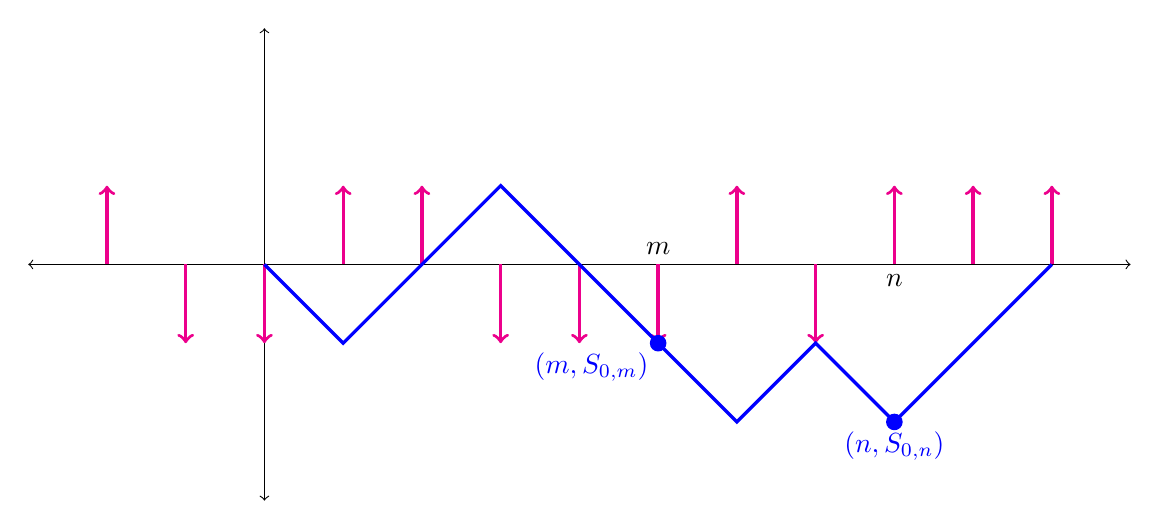
\begin{tikzpicture}
        \draw[<->] (-3,0)--(11,0);
        \draw[<->] (0,-3)--(0,3);
        \foreach \i in {-2,1,2,6,8,9,10}{
            \draw[->,very thick, magenta] (\i,0)--(\i,1);
            };
        \foreach \i in {-1,0,3,4,5,7}{
            \draw[->, very thick, magenta] (\i,0)--(\i,-1);
            };
        \draw[blue, very thick] (0,0) -- (1,-1) -- (2,0) -- (3,1) -- (4,0)
            -- (5,-1) -- (6,-2) -- (7,-1) -- (8,-2) -- (9,-1) -- (10,0);
        \node at (5,0.2) {$m$};
        \node at (8,-0.2) {$n$};
        \fill[blue] (5,-1) circle (3pt) node[below left] {$(m,S_{0,m})$};
        \fill[blue] (8,-2) circle (3pt) node[below] {$(n,S_{0,n})$};
    \end{tikzpicture}
    }
\hfil
\resizebox{0.45\textwidth}{!}{
    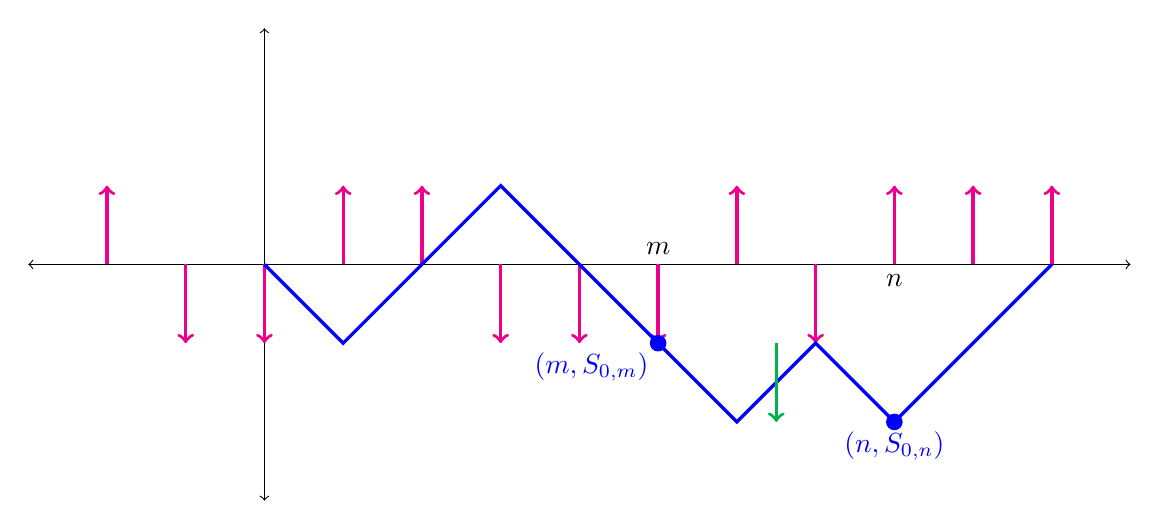
\begin{tikzpicture}
        \draw[<->] (-3,0)--(11,0);
        \draw[<->] (0,-3)--(0,3);
        \foreach \i in {-2,1,2,6,8,9,10}{
            \draw[->,very thick, magenta] (\i,0)--(\i,1);
            };
        \foreach \i in {-1,0,3,4,5,7}{
            \draw[->, very thick, magenta] (\i,0)--(\i,-1);
            };
        \draw[blue, very thick] (0,0) -- (1,-1) -- (2,0) -- (3,1) -- (4,0)
            -- (5,-1) -- (6,-2) -- (7,-1) -- (8,-2) -- (9,-1) -- (10,0);
        \node at (5,0.2) {$m$};
        \node at (8,-0.2) {$n$};
        \fill[blue] (5,-1) circle (3pt) node[below left] {$(m,S_{0,m})$};
        \fill[blue] (8,-2) circle (3pt) node[below] {$(n,S_{0,n})$};
        \draw[green!70!blue, ->, very thick] (6.5,-1)--(6.5,-2);
    \end{tikzpicture}
    }
\hfil
\caption{Illustrations of $S_{0, m}$, $S_{0, n}$ and $S_{m, n-m}$}
\end{figure}


% ======= Hard formatting!

\filbreak

% ======= Hard formatting!


This gives a visualization of the fact that for $n\geq m$,
\begin{equation*}
    S_{0, n} = S_{0, m} + S_{m, n-m}\,.
\end{equation*}
Similarly, we can visualize $\{S_{-2, n}\}_{n=1, 2, \ldots}$.
The portion of the blue curve that's on the right half
    of the vertical axis is the same as in the pictures above,
    since $S_{-2, 2}=0$.
%\begin{center}
%\begin{tikzpicture}
%    \draw[<->] (-3,0)--(11,0);
%    \draw[<->] (0,-4)--(0,4);
%    \foreach \i in {-2,1,2,6,8,9,10}{
%        \draw[->,very thick, magenta] (\i,0)--(\i,1);
%        };
%    \foreach \i in {-1,0,3,4,5,7}{
%        \draw[->, very thick, magenta] (\i,0)--(\i,-1);
%        };
%    \draw[blue, very thick] (0,0) -- (1,-1) -- (2,0) -- (3,1) -- (4,0)
%        -- (5,-1) -- (6,-2) -- (7,-1) -- (8,-2) -- (9,-1) -- (10,0);
%    \node at (5,0.2) {$m$};
%    \node at (7,0.2) {$n$};
%    \fill[blue] (5,-1) circle (3pt) node[below left] {$(m,S_{0,m})$};
%    \fill[blue] (7,-1);
%\end{tikzpicture}
%\end{center}


Observe that $\var[S_{0, n}] = n$,
    which can be used to show the more general statement that for $m \leq n$,
    $\cov[S_{0, m}, S_{0, n}] = m$.
This comes from the following chain of equalities:
\begin{align*}
\cov[S_{0, m},S_{0, n}] &= \cov[S_{0, m},S_{0, m} + S_{m, n-m}]\\
                        &= \cov[S_{0, m}, S_{0, m}] + \cov[S_{0, m}, S_{m, n-m}]
                            &\text{since $\cov$ is bilinear}\\
                        &= m + 0 
                            &\text{since $S_{0, m}$ and $S_{m, n-m}$
                                    are independent}\\
                        &= m.
\end{align*}


Note that Equation 1\addref\ holds in the more general case that
    $\E[Z]=0$ and $\var[Z] = 1$.


\section{Brownian Motion}


Let $S_{k, n}$ be defined as above and
\begin{equation*} 
    B_t^{(N)} = \frac{1}{\sqrt{N}} S_{0, \lfloor t N\rfloor}\,.
\end{equation*}
Then let
\begin{equation*}
    B_t = \lim_{N \to \infty} \frac{1}{\sqrt{N}} S_{0, \lfloor t N\rfloor}
\end{equation*}
Then $\{B_t\}$ is a \defn{Brownian motion}.
We can visualize Brownian motion by considering the graphs
    yielded by the maps $t \mapsto B^t$ and $t\mapsto B_t^{(N)}$.


For example,
    if we let $N = 25$, the function $t \mapsto B_t^{(N)}$ 
    yields the following graph for $t=0$ to $t=10$,
    for a particular sequence $\{X_k\}_{k \in {\mathbb{Z}_{\geq 0}}}$.
\begin{figure}[h]
\resizebox{\textwidth}{!}{
    \begin{tikzpicture}
        \draw[<->] (-1,0)--(11,0);
        \draw[<->] (0,-3)--(0,3);
        \foreach \i in {-2,-1,1,2}{
            \draw[-] (0.2,\i)--(-0.2,\i) node[left] {$\i$};
            \draw[-] (10,0.2)--(10,-0.2) node[below] {$10$};
            };
        \draw[-,very thick](0.0, 0.0)--(0.04, 0.0);
        \draw[-,very thick](0.04, 0.2)--(0.08, 0.2);
        \draw[-,very thick](0.08, 0.4)--(0.12, 0.4);
        \draw[-,very thick](0.12, 0.2)--(0.16, 0.2);
        \draw[-,very thick](0.16, 0.0)--(0.2, 0.0);
        \draw[-,very thick](0.2, -0.2)--(0.24, -0.2);
        \draw[-,very thick](0.24, 0.0)--(0.28, 0.0);
        \draw[-,very thick](0.28, -0.2)--(0.32, -0.2);
        \draw[-,very thick](0.32, -0.4)--(0.36, -0.4);
        \draw[-,very thick](0.36, -0.2)--(0.4, -0.2);
        \draw[-,very thick](0.4, -0.4)--(0.44, -0.4);
        \draw[-,very thick](0.44, -0.6)--(0.48, -0.6);
        \draw[-,very thick](0.48, -0.4)--(0.52, -0.4);
        \draw[-,very thick](0.52, -0.6)--(0.56, -0.6);
        \draw[-,very thick](0.56, -0.4)--(0.6, -0.4);
        \draw[-,very thick](0.6, -0.6)--(0.64, -0.6);
        \draw[-,very thick](0.64, -0.4)--(0.68, -0.4);
        \draw[-,very thick](0.68, -0.6)--(0.72, -0.6);
        \draw[-,very thick](0.72, -0.8)--(0.76, -0.8);
        \draw[-,very thick](0.76, -0.6)--(0.8, -0.6);
        \draw[-,very thick](0.8, -0.8)--(0.84, -0.8);
        \draw[-,very thick](0.84, -1.0)--(0.88, -1.0);
        \draw[-,very thick](0.88, -0.8)--(0.92, -0.8);
        \draw[-,very thick](0.92, -0.6)--(0.96, -0.6);
        \draw[-,very thick](0.96, -0.8)--(1.0, -0.8);
        \draw[-,very thick](1.0, -1.0)--(1.04, -1.0);
        \draw[-,very thick](1.04, -0.8)--(1.08, -0.8);
        \draw[-,very thick](1.08, -0.6)--(1.12, -0.6);
        \draw[-,very thick](1.12, -0.8)--(1.16, -0.8);
        \draw[-,very thick](1.16, -0.6)--(1.2, -0.6);
        \draw[-,very thick](1.2, -0.8)--(1.24, -0.8);
        \draw[-,very thick](1.24, -0.6)--(1.28, -0.6);
        \draw[-,very thick](1.28, -0.8)--(1.32, -0.8);
        \draw[-,very thick](1.32, -1.0)--(1.36, -1.0);
        \draw[-,very thick](1.36, -1.2)--(1.4, -1.2);
        \draw[-,very thick](1.4, -1.4)--(1.44, -1.4);
        \draw[-,very thick](1.44, -1.6)--(1.48, -1.6);
        \draw[-,very thick](1.48, -1.4)--(1.52, -1.4);
        \draw[-,very thick](1.52, -1.2)--(1.56, -1.2);
        \draw[-,very thick](1.56, -1.4)--(1.6, -1.4);
        \draw[-,very thick](1.6, -1.6)--(1.64, -1.6);
        \draw[-,very thick](1.64, -1.4)--(1.68, -1.4);
        \draw[-,very thick](1.68, -1.6)--(1.72, -1.6);
        \draw[-,very thick](1.72, -1.4)--(1.76, -1.4);
        \draw[-,very thick](1.76, -1.2)--(1.8, -1.2);
        \draw[-,very thick](1.8, -1.4)--(1.84, -1.4);
        \draw[-,very thick](1.84, -1.2)--(1.88, -1.2);
        \draw[-,very thick](1.88, -1.4)--(1.92, -1.4);
        \draw[-,very thick](1.92, -1.2)--(1.96, -1.2);
        \draw[-,very thick](1.96, -1.0)--(2.0, -1.0);
        \draw[-,very thick](2.0, -0.8)--(2.04, -0.8);
        \draw[-,very thick](2.04, -0.6)--(2.08, -0.6);
        \draw[-,very thick](2.08, -0.4)--(2.12, -0.4);
        \draw[-,very thick](2.12, -0.2)--(2.16, -0.2);
        \draw[-,very thick](2.16, 0.0)--(2.2, 0.0);
        \draw[-,very thick](2.2, 0.2)--(2.24, 0.2);
        \draw[-,very thick](2.24, 0.4)--(2.28, 0.4);
        \draw[-,very thick](2.28, 0.6)--(2.32, 0.6);
        \draw[-,very thick](2.32, 0.4)--(2.36, 0.4);
        \draw[-,very thick](2.36, 0.2)--(2.4, 0.2);
        \draw[-,very thick](2.4, 0.0)--(2.44, 0.0);
        \draw[-,very thick](2.44, 0.2)--(2.48, 0.2);
        \draw[-,very thick](2.48, 0.0)--(2.52, 0.0);
        \draw[-,very thick](2.52, -0.2)--(2.56, -0.2);
        \draw[-,very thick](2.56, 0.0)--(2.6, 0.0);
        \draw[-,very thick](2.6, 0.2)--(2.64, 0.2);
        \draw[-,very thick](2.64, 0.4)--(2.68, 0.4);
        \draw[-,very thick](2.68, 0.6)--(2.72, 0.6);
        \draw[-,very thick](2.72, 0.4)--(2.76, 0.4);
        \draw[-,very thick](2.76, 0.2)--(2.8, 0.2);
        \draw[-,very thick](2.8, 0.0)--(2.84, 0.0);
        \draw[-,very thick](2.84, -0.2)--(2.88, -0.2);
        \draw[-,very thick](2.88, -0.4)--(2.92, -0.4);
        \draw[-,very thick](2.92, -0.2)--(2.96, -0.2);
        \draw[-,very thick](2.96, 0.0)--(3.0, 0.0);
        \draw[-,very thick](3.0, -0.2)--(3.04, -0.2);
        \draw[-,very thick](3.04, 0.0)--(3.08, 0.0);
        \draw[-,very thick](3.08, -0.2)--(3.12, -0.2);
        \draw[-,very thick](3.12, 0.0)--(3.16, 0.0);
        \draw[-,very thick](3.16, 0.2)--(3.2, 0.2);
        \draw[-,very thick](3.2, 0.4)--(3.24, 0.4);
        \draw[-,very thick](3.24, 0.6)--(3.28, 0.6);
        \draw[-,very thick](3.28, 0.8)--(3.32, 0.8);
        \draw[-,very thick](3.32, 1.0)--(3.36, 1.0);
        \draw[-,very thick](3.36, 0.8)--(3.4, 0.8);
        \draw[-,very thick](3.4, 0.6)--(3.44, 0.6);
        \draw[-,very thick](3.44, 0.4)--(3.48, 0.4);
        \draw[-,very thick](3.48, 0.6)--(3.52, 0.6);
        \draw[-,very thick](3.52, 0.8)--(3.56, 0.8);
        \draw[-,very thick](3.56, 0.6)--(3.6, 0.6);
        \draw[-,very thick](3.6, 0.4)--(3.64, 0.4);
        \draw[-,very thick](3.64, 0.6)--(3.68, 0.6);
        \draw[-,very thick](3.68, 0.4)--(3.72, 0.4);
        \draw[-,very thick](3.72, 0.6)--(3.76, 0.6);
        \draw[-,very thick](3.76, 0.8)--(3.8, 0.8);
        \draw[-,very thick](3.8, 0.6)--(3.84, 0.6);
        \draw[-,very thick](3.84, 0.8)--(3.88, 0.8);
        \draw[-,very thick](3.88, 0.6)--(3.92, 0.6);
        \draw[-,very thick](3.92, 0.4)--(3.96, 0.4);
        \draw[-,very thick](3.96, 0.6)--(4.0, 0.6);
        \draw[-,very thick](4.0, 0.4)--(4.04, 0.4);
        \draw[-,very thick](4.04, 0.2)--(4.08, 0.2);
        \draw[-,very thick](4.08, 0.4)--(4.12, 0.4);
        \draw[-,very thick](4.12, 0.6)--(4.16, 0.6);
        \draw[-,very thick](4.16, 0.4)--(4.2, 0.4);
        \draw[-,very thick](4.2, 0.6)--(4.24, 0.6);
        \draw[-,very thick](4.24, 0.4)--(4.28, 0.4);
        \draw[-,very thick](4.28, 0.6)--(4.32, 0.6);
        \draw[-,very thick](4.32, 0.8)--(4.36, 0.8);
        \draw[-,very thick](4.36, 1.0)--(4.4, 1.0);
        \draw[-,very thick](4.4, 0.8)--(4.44, 0.8);
        \draw[-,very thick](4.44, 0.6)--(4.48, 0.6);
        \draw[-,very thick](4.48, 0.4)--(4.52, 0.4);
        \draw[-,very thick](4.52, 0.6)--(4.56, 0.6);
        \draw[-,very thick](4.56, 0.8)--(4.6, 0.8);
        \draw[-,very thick](4.6, 1.0)--(4.64, 1.0);
        \draw[-,very thick](4.64, 1.2)--(4.68, 1.2);
        \draw[-,very thick](4.68, 1.4)--(4.72, 1.4);
        \draw[-,very thick](4.72, 1.2)--(4.76, 1.2);
        \draw[-,very thick](4.76, 1.4)--(4.8, 1.4);
        \draw[-,very thick](4.8, 1.2)--(4.84, 1.2);
        \draw[-,very thick](4.84, 1.4)--(4.88, 1.4);
        \draw[-,very thick](4.88, 1.6)--(4.92, 1.6);
        \draw[-,very thick](4.92, 1.4)--(4.96, 1.4);
        \draw[-,very thick](4.96, 1.2)--(5.0, 1.2);
        \draw[-,very thick](5.0, 1.0)--(5.04, 1.0);
        \draw[-,very thick](5.04, 0.8)--(5.08, 0.8);
        \draw[-,very thick](5.08, 0.6)--(5.12, 0.6);
        \draw[-,very thick](5.12, 0.8)--(5.16, 0.8);
        \draw[-,very thick](5.16, 0.6)--(5.2, 0.6);
        \draw[-,very thick](5.2, 0.8)--(5.24, 0.8);
        \draw[-,very thick](5.24, 0.6)--(5.28, 0.6);
        \draw[-,very thick](5.28, 0.8)--(5.32, 0.8);
        \draw[-,very thick](5.32, 1.0)--(5.36, 1.0);
        \draw[-,very thick](5.36, 1.2)--(5.4, 1.2);
        \draw[-,very thick](5.4, 1.4)--(5.44, 1.4);
        \draw[-,very thick](5.44, 1.6)--(5.48, 1.6);
        \draw[-,very thick](5.48, 1.4)--(5.52, 1.4);
        \draw[-,very thick](5.52, 1.2)--(5.56, 1.2);
        \draw[-,very thick](5.56, 1.0)--(5.6, 1.0);
        \draw[-,very thick](5.6, 0.8)--(5.64, 0.8);
        \draw[-,very thick](5.64, 0.6)--(5.68, 0.6);
        \draw[-,very thick](5.68, 0.4)--(5.72, 0.4);
        \draw[-,very thick](5.72, 0.6)--(5.76, 0.6);
        \draw[-,very thick](5.76, 0.8)--(5.8, 0.8);
        \draw[-,very thick](5.8, 0.6)--(5.84, 0.6);
        \draw[-,very thick](5.84, 0.4)--(5.88, 0.4);
        \draw[-,very thick](5.88, 0.2)--(5.92, 0.2);
        \draw[-,very thick](5.92, 0.4)--(5.96, 0.4);
        \draw[-,very thick](5.96, 0.2)--(6.0, 0.2);
        \draw[-,very thick](6.0, 0.4)--(6.04, 0.4);
        \draw[-,very thick](6.04, 0.2)--(6.08, 0.2);
        \draw[-,very thick](6.08, 0.0)--(6.12, 0.0);
        \draw[-,very thick](6.12, -0.2)--(6.16, -0.2);
        \draw[-,very thick](6.16, -0.4)--(6.2, -0.4);
        \draw[-,very thick](6.2, -0.2)--(6.24, -0.2);
        \draw[-,very thick](6.24, 0.0)--(6.28, 0.0);
        \draw[-,very thick](6.28, 0.2)--(6.32, 0.2);
        \draw[-,very thick](6.32, 0.0)--(6.36, 0.0);
        \draw[-,very thick](6.36, -0.2)--(6.4, -0.2);
        \draw[-,very thick](6.4, -0.4)--(6.44, -0.4);
        \draw[-,very thick](6.44, -0.6)--(6.48, -0.6);
        \draw[-,very thick](6.48, -0.4)--(6.52, -0.4);
        \draw[-,very thick](6.52, -0.2)--(6.56, -0.2);
        \draw[-,very thick](6.56, -0.4)--(6.6, -0.4);
        \draw[-,very thick](6.6, -0.6)--(6.64, -0.6);
        \draw[-,very thick](6.64, -0.4)--(6.68, -0.4);
        \draw[-,very thick](6.68, -0.2)--(6.72, -0.2);
        \draw[-,very thick](6.72, -0.4)--(6.76, -0.4);
        \draw[-,very thick](6.76, -0.6)--(6.8, -0.6);
        \draw[-,very thick](6.8, -0.4)--(6.84, -0.4);
        \draw[-,very thick](6.84, -0.6)--(6.88, -0.6);
        \draw[-,very thick](6.88, -0.8)--(6.92, -0.8);
        \draw[-,very thick](6.92, -0.6)--(6.96, -0.6);
        \draw[-,very thick](6.96, -0.8)--(7.0, -0.8);
        \draw[-,very thick](7.0, -1.0)--(7.04, -1.0);
        \draw[-,very thick](7.04, -0.8)--(7.08, -0.8);
        \draw[-,very thick](7.08, -0.6)--(7.12, -0.6);
        \draw[-,very thick](7.12, -0.4)--(7.16, -0.4);
        \draw[-,very thick](7.16, -0.2)--(7.2, -0.2);
        \draw[-,very thick](7.2, -0.4)--(7.24, -0.4);
        \draw[-,very thick](7.24, -0.2)--(7.28, -0.2);
        \draw[-,very thick](7.28, 0.0)--(7.32, 0.0);
        \draw[-,very thick](7.32, -0.2)--(7.36, -0.2);
        \draw[-,very thick](7.36, 0.0)--(7.4, 0.0);
        \draw[-,very thick](7.4, -0.2)--(7.44, -0.2);
        \draw[-,very thick](7.44, -0.4)--(7.48, -0.4);
        \draw[-,very thick](7.48, -0.6)--(7.52, -0.6);
        \draw[-,very thick](7.52, -0.8)--(7.56, -0.8);
        \draw[-,very thick](7.56, -1.0)--(7.6, -1.0);
        \draw[-,very thick](7.6, -1.2)--(7.64, -1.2);
        \draw[-,very thick](7.64, -1.0)--(7.68, -1.0);
        \draw[-,very thick](7.68, -1.2)--(7.72, -1.2);
        \draw[-,very thick](7.72, -1.0)--(7.76, -1.0);
        \draw[-,very thick](7.76, -0.8)--(7.8, -0.8);
        \draw[-,very thick](7.8, -0.6)--(7.84, -0.6);
        \draw[-,very thick](7.84, -0.4)--(7.88, -0.4);
        \draw[-,very thick](7.88, -0.6)--(7.92, -0.6);
        \draw[-,very thick](7.92, -0.8)--(7.96, -0.8);
        \draw[-,very thick](7.96, -0.6)--(8.0, -0.6);
        \draw[-,very thick](8.0, -0.8)--(8.04, -0.8);
        \draw[-,very thick](8.04, -0.6)--(8.08, -0.6);
        \draw[-,very thick](8.08, -0.4)--(8.12, -0.4);
        \draw[-,very thick](8.12, -0.6)--(8.16, -0.6);
        \draw[-,very thick](8.16, -0.8)--(8.2, -0.8);
        \draw[-,very thick](8.2, -1.0)--(8.24, -1.0);
        \draw[-,very thick](8.24, -0.8)--(8.28, -0.8);
        \draw[-,very thick](8.28, -1.0)--(8.32, -1.0);
        \draw[-,very thick](8.32, -1.2)--(8.36, -1.2);
        \draw[-,very thick](8.36, -1.0)--(8.4, -1.0);
        \draw[-,very thick](8.4, -1.2)--(8.44, -1.2);
        \draw[-,very thick](8.44, -1.0)--(8.48, -1.0);
        \draw[-,very thick](8.48, -1.2)--(8.52, -1.2);
        \draw[-,very thick](8.52, -1.0)--(8.56, -1.0);
        \draw[-,very thick](8.56, -1.2)--(8.6, -1.2);
        \draw[-,very thick](8.6, -1.0)--(8.64, -1.0);
        \draw[-,very thick](8.64, -1.2)--(8.68, -1.2);
        \draw[-,very thick](8.68, -1.0)--(8.72, -1.0);
        \draw[-,very thick](8.72, -1.2)--(8.76, -1.2);
        \draw[-,very thick](8.76, -1.4)--(8.8, -1.4);
        \draw[-,very thick](8.8, -1.2)--(8.84, -1.2);
        \draw[-,very thick](8.84, -1.0)--(8.88, -1.0);
        \draw[-,very thick](8.88, -0.8)--(8.92, -0.8);
        \draw[-,very thick](8.92, -1.0)--(8.96, -1.0);
        \draw[-,very thick](8.96, -0.8)--(9.0, -0.8);
        \draw[-,very thick](9.0, -0.6)--(9.04, -0.6);
        \draw[-,very thick](9.04, -0.8)--(9.08, -0.8);
        \draw[-,very thick](9.08, -0.6)--(9.12, -0.6);
        \draw[-,very thick](9.12, -0.8)--(9.16, -0.8);
        \draw[-,very thick](9.16, -1.0)--(9.2, -1.0);
        \draw[-,very thick](9.2, -0.8)--(9.24, -0.8);
        \draw[-,very thick](9.24, -0.6)--(9.28, -0.6);
        \draw[-,very thick](9.28, -0.4)--(9.32, -0.4);
        \draw[-,very thick](9.32, -0.6)--(9.36, -0.6);
        \draw[-,very thick](9.36, -0.8)--(9.4, -0.8);
        \draw[-,very thick](9.4, -1.0)--(9.44, -1.0);
        \draw[-,very thick](9.44, -1.2)--(9.48, -1.2);
        \draw[-,very thick](9.48, -1.4)--(9.52, -1.4);
        \draw[-,very thick](9.52, -1.2)--(9.56, -1.2);
        \draw[-,very thick](9.56, -1.0)--(9.6, -1.0);
        \draw[-,very thick](9.6, -1.2)--(9.64, -1.2);
        \draw[-,very thick](9.64, -1.4)--(9.68, -1.4);
        \draw[-,very thick](9.68, -1.2)--(9.72, -1.2);
        \draw[-,very thick](9.72, -1.4)--(9.76, -1.4);
        \draw[-,very thick](9.76, -1.2)--(9.8, -1.2);
        \draw[-,very thick](9.8, -1.4)--(9.84, -1.4);
        \draw[-,very thick](9.84, -1.6)--(9.88, -1.6);
        \draw[-,very thick](9.88, -1.8)--(9.92, -1.8);
        \draw[-,very thick](9.92, -2.0)--(9.96, -2.0);
        \draw[-,very thick](9.96, -2.2)--(10.0, -2.2);
        \draw[-,very thick](10.0, -2.4)--(10.04, -2.4);
    \end{tikzpicture}
    }
\caption{Plot of a Brownian motion with $N = 25$ and $0 \leq t \leq 10$}
\end{figure}


% ======= Hard formatting!

\filbreak

% ======= Hard formatting!


The Central Limit Theorem tells us that $B_t - B_s \sim N(0, t - s)$.  
Additionally,
\begin{equation*}
    \var[B_t] = \lim_{N \to \infty} \dfrac{\lfloor t N\rfloor}{N} = t
\end{equation*} 
and
\begin{equation*}
    \cov[B_s, B_t] = s
\end{equation*}
    for $s \leq t$.


\begin{definition}
A \defn{standard Brownian motion} is a stochastic process $\{B_t\}_{t \geq 0}$
    such that
\begin{enumerate}[(i)]
    \item $B_0 = 0$
    \item $B_t - B_s \sim N(0, t - s)$---that is,
        the variance of an increment is proportional to the time difference
    \item $B_t - B_s$ is independent of $B_v - B_u$ for $u < v \leq s < t$ 
\end{enumerate}
\end{definition}


That is, Brownian motion is
    the stochastic process with independent Gaussian increments,
    ie. how it moves in an interval just depends
        on the length of that interval, not the interval itself.


\begin{example}
Suppose a stream of energetic particles is absorbed by some object
    and the energy is slowly released from that object.
Suppose at time $t$,
    the proportion of energy that remains in the object
    from a particle absorbed $t$ time units ago is $e^{-t}$.
Assuming that the object only absorbs energy at times $t = 0, 1, 2, \ldots$,
    let $X_t$ be the amount of energy absorbed at time $t$.
Let $Z_n$ be the total energy contained in the object at time $n$.
Then
\begin{equation*}
    Z_n = \sum_{k = 0}^\infty e^{-k}X_{n - k}\,.
\end{equation*}
We can scale the $x$ and $y$ axes: let
\begin{equation*}
    Z_{\lfloor t N\rfloor} = \frac{1}{\sqrt{N}} \sum_{k=0}^\infty
         e^{-k/N}X_{\lfloor t N\rfloor - k}.
\end{equation*}
Then
\begin{equation*}
    Z_{\lfloor t N\rfloor}\xrightarrow{N \to \infty} Z_t\,.
\end{equation*}
\end{example}


% ==============================================================================
%
\end{document}
%
% ==============================================================================
